\documentclass[14pt]{article}
\usepackage{listings}
\usepackage{color}
\usepackage{graphicx}
\usepackage{setspace}
\usepackage{algorithm}
\usepackage{amssymb}
\usepackage{amsmath}
\usepackage[noend]{algpseudocode}

\definecolor{dkgreen}{rgb}{0,0.6,0}
\definecolor{gray}{rgb}{0.5,0.5,0.5}
\definecolor{mauve}{rgb}{0.58,0,0.82}

\lstset{frame=tb,
  language=C,
  aboveskip=3mm,
  belowskip=3mm,
  showstringspaces=false,
  columns=flexible,
  basicstyle={\small\ttfamily},
  numbers=none,
  numberstyle=\tiny\color{gray},
  keywordstyle=\color{blue},
  commentstyle=\color{dkgreen},
  stringstyle=\color{mauve},
  breaklines=true,
  breakatwhitespace=true
  tabsize=3
}







\begin{document}
\title{\huge The Shortest Path in a Graph}
\date{\today}
\maketitle
\begin{center}
\vspace{30 mm}

\title{\huge Student: Popa Radu - Mircea}
\\\vspace{10 mm}
\title{\huge Computers and Information Technology (in English)}
\\\vspace{10 mm}
\title{\huge CEN 1.2 B}
\\\vspace{10 mm}
\title{\huge 1st Year}
\date{}
\maketitle

\newpage
\end{center}
\section*{Problem statement}
George is a truck driver, he needs to transport cargo from Craiova to Paris in a given limited amount of time. Write an application that allows George to establish the shortest route, with given source and destination points. Also, all the connections between the points on the map are given. The
application should implement two different algorithms to solve the above problem.
\begin{center}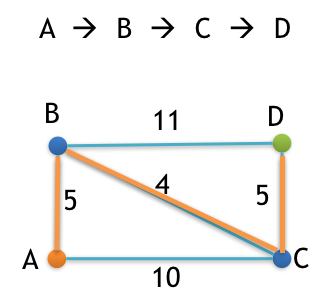
\includegraphics[height=3.5in, width = 3.5in]{graf.jpg}
\end{center}

\newpage
\section*{Introduction}
\vspace{20 mm}
Dijkstra's algorithm is an algorithm for finding the shortest paths between nodes in a graph, which may represent, for example, road networks. Dijkstra's original algorithm runs in time ${\displaystyle O(|V|^{2})}$ (where ${\displaystyle |V|}$ is the number of nodes).
\\\vspace{10 mm}
\\
The Floyd Warshall algorithm is an algorithm for finding shortest paths in a weighted graph. The Floyd Warshall algorithm compares all possible paths through the graph.  It is able to do this with ${\displaystyle \Theta (|V|^{3})}$ comparisons in a graph.  



\newpage
\section*{Pseudocode}
We will use an adjacency matrix for the graph representation, generated randomly with the random generator program. 
\\
We will use functions for each operation required by the application, with integer parameters, which will be called by the main program.
\\
Here are the important functions employed by the program:
\begin{lstlisting}
floyd(int graph[][V])
//V is the number of nodes, generated randomly. Change this value every time, in all the files!
1.	for i<-0,V do
2.	    for j<-0,V do
3.	        dist[i][j] <- graph[i][j]
3.          pred[i][j] <- i
4.	for k<-0,V do
5.      for i<-0,V do
6.          if dist[i][j] > dist[i][k] + dist[k][j] then
7.      dist[i][j] <- dist[i][k] + dist[k][j]
8.      pred[i][j] <- k
9.   print path
\end{lstlisting}
\begin{lstlisting}
dijkstra(int graph[V][V], int source, int destination)
1.	for r<-0,V do
2.	    for c<-0,V do
3.	        weightTable[r][c] <- INF
4.	weightTable[wtTableR++][source] <- 0
5.	markedNodes[markedNodesIndex++] <- source
6.	currVertex <- source  
7.	while currVertex != currentVertex and not(checkMarked(c, markedNodes, markedNodesIndex)) do
8.	    edgeWt <- graph[currVertex][c]
9.		destValue <- weightTable[wtTableR - 1][c]
10.		markedValue <- weightTable[wtTableR][currVertex]
11.		find min between destValue and markedValue + edgeWt
12.	    weightTable[wtTableR][c] <- min
13.	    min <- INF
14.     for c<-0,V do
15.      if not(checkMarked(c, markedNodes, markedNodesIndex) then
16.         if weightTable[wtTableR][c] < min then
17.             min <- weightTable[wtTableR][c]
18.             temp <- c
19.     markedNodes[markedNodesIndex++] <- tempC
20.     currVertex <- tempC
21.     wtTableR++
22. c <- destination
23. shortestPathNodes[shortestPathNodesIndex++] <- c
24. markedValue <- weightTable[wtTableR - 1][destination]
25. for r<-wtTableR - 2,0 do
26.     if weightTable[r][c] != markedValue then
27.         c <- markedNodes[r]
28.         markedValue <- weightTable[r][c]
29.         shortestPathNodes[shortestPathNodesIndex++] <- c
30. Display the shortest path and its weight
\end{lstlisting}




\newpage
\section*{Application design}
\vspace{10 mm}
The application contains the header \textbf{\textit{functions.h}} which has all the function prototypes to compute the required operations. These are all of them:
\\---void findpath( int u, int v, int dist[][V], int pred[][V] )
\\---void printpath( int dist[][V], int pred[][V] )
\\---void floyd( int graph[][V] )
\\---int findMin( int x, int y )
\\---int checkMarked( int n, int markedNodes[], int markedNodesIndex )
\\---void dijkstra( int graph[V][V], int source, int destination )

\\\vspace{3 mm}
\\The source file \textbf{\textit{functions.c}} has all the function implementations.
\\The function findMin( int x, int y ) returns the minimum value between two numbers.
\\The function checkMarked( int n, int markedNodes[], int markedNodesIndex ) checks if the vertex is marked.
\\\ For more details about the functions used, such as the parameters used, see the Doxy generated documentation!
\\\vspace{3 mm}
\\Dijstra Algorithm:
\\ Let the node at which we are starting be called the initial node. Let the distance of node Y be the distance from the initial node to Y. Dijkstra's algorithm will assign some initial distance values and will try to improve them step by step.

Mark all nodes unvisited. Create a set of all the unvisited nodes called the unvisited set.
Assign to every node a tentative distance value: set it to zero for our initial node and to infinity for all other nodes. Set the initial node as current.
For the current node, consider all of its unvisited neighbors and calculate their tentative distances through the current node. Compare the newly calculated tentative distance to the current assigned value and assign the smaller one. For example, if the current node A is marked with a distance of 6, and the edge connecting it with a neighbor B has length 2, then the distance to B through A will be 6 + 2 = 8. If B was previously marked with a distance greater than 8 then change it to 8. Otherwise, keep the current value.
When we are done considering all of the unvisited neighbors of the current node, mark the current node as visited and remove it from the unvisited set. A visited node will never be checked again.
Move to the next unvisited node with the smallest tentative distance and repeat the above steps which check neighbors and mark visited.
If the destination node has been marked visited (when planning a route between two specific nodes) or if the smallest tentative distance among the nodes in the unvisited set is infinity (when planning a complete traversal; occurs when there is no connection between the initial node and remaining unvisited nodes), then stop. The algorithm has finished.
Otherwise, select the unvisited node that is marked with the smallest tentative distance, set it as the new "current node", and go back to step 3.
\\\vspace{2 mm}
\\

\newpage
\section*{Source Code}
\begin{lstlisting}
//-----------------------------functions.h-------------------------------

///\file functions.h
///\brief This header file contains all the required
///definitions of the functions used in Dijkstra Algorithm.
///\author Radu Popa
///\date 05.06.2018.

#define MAIN_H_INCLUDED

#include <stdio.h>
#define INF 0x3fffffff
#define V 6
///\def #define V 6
///\brief The number of nodes. Don't forget to change this number with the one generated randomly!

void find_path( int u, int v, int dist[][V], int pred[][V] );
void print_path( int dist[][V], int pred[][V] );
void floyd( int graph[][V] );

//-------------------
///\file functions.h
///\brief This header file contains all the required
///definitions of the functions used in Dijkstra Algorithm.
///\author Radu Popa
///\date 05.06.2018.


#define MAIN_H_INCLUDED

#include <stdio.h>
#define V 6
///\def #define V 6
///\brief The number of nodes. Don't forget to change this number with the one generated randomly!

int findMin( int x, int y );
int checkMarked( int n, int markedNodes[], int markedNodesIndex );
void dijkstra( int graph[V][V], int source, int destination );



\end{lstlisting}
\begin{lstlisting}
//-----------------------------functions.c-------------------------------

///\file functions.c
///\brief This file contains all the functions needed
///in Dijkstra Algorithm to find the shortest path between two nodes.
///
///\author Radu Popa
///\date 6/05/2018

#include "functions.h"
#define INF 0x3fffffff
#define V 6
///\def #define V 6
///\brief The number of nodes. Don't forget to change this number with the one generated randomly!
///\def #define INF 0x3fffffff
///\brief A constant to represent infinity. It is assumed that no edge will have this weight.

int findMin( int x, int y ){
    ///\fn int findMin( int x, int y )
    ///\brief This function returns the minimum value between two numbers.
    ///\param a First integer
    ///\param b Second integer
    ///
    if( x < y ){
        return x;
    }
    return y;
}

int checkMarked( int n, int markedNodes[], int markedNodesIndex ){
    ///\fn int checkMarked( int n, int markedNodes[], int markedNodesIndex )
    ///\brief This function checks if the vertex is marked.
    ///\param v integer
    ///\param markedNodes[] array of integers
    ///\param markedNodesIndex integer
    int iterator = 0;
    for( iterator = 0; iterator < markedNodesIndex; iterator++ ){
        if( n == markedNodes[iterator] ){
            return 1;
        }
    }
    return 0;
}

void dijkstra( int graph[V][V], int source, int destination ){
    ///\fn void dijkstra( int graph[V][V], int source, int destination )
    ///\brief This function finds the shortest path between the source and the destination nodes.
    ///\param graph[][] matrix
    ///\param source integer
    ///\param destination integer
    ///variables
    int i;
    int r;
    int c;
    int tempC;
    int min;
    int currVertex;
    int edgeWt = 0;
    int destValue = 0;
    int markedValue = 0;
    int wtTableR = 0;
    int markedNodesIndex = 0;

    ///array containing vertices in the shortest path
    int shortestPathNodes[V] = {-1};
    int shortestPathNodesIndex = 0;

    ///this matrix stores the weight of the edges
    int weightTable[V][V];
    for( r = 0; r < V; r++ ){
        for( c = 0; c < V; c++ ){
            weightTable[r][c] = INF;
        }
    }
    weightTable[wtTableR++][source] = 0;

    ///nodes that are marked
    int markedNodes[V] = {-1};
    markedNodes[markedNodesIndex++] = source;
    currVertex = source;

    ///find the shortest path
    while( currVertex != destination ){
        ///copy the marked values to the next row of weightTable
        for( i = 0; i < markedNodesIndex; i++ ){
            c = markedNodes[i];
            weightTable[wtTableR][c] = weightTable[wtTableR - 1][c];
        }
        ///find the weight from the current node to all he other
        ///nodes that are directly connected and not yet marked
        for( c = 0; c < V; c++ ){
            if( c != currVertex && !checkMarked(c, markedNodes, markedNodesIndex) ){
                edgeWt = graph[currVertex][c];
                destValue = weightTable[wtTableR - 1][c];
                markedValue = weightTable[wtTableR][currVertex];

                min = findMin( destValue, markedValue + edgeWt );

                weightTable[wtTableR][c] = min;
            }
        }

        ///find the minimum unmarked nodes on the current row
        min = INF;
        for( c = 0; c < V; c++ ){
            if( !checkMarked(c, markedNodes, markedNodesIndex) ){
                if( weightTable[wtTableR][c] < min ){
                    min = weightTable[wtTableR][c];
                    tempC = c;
                }
            }
            
        }

        ///found a node to be marked
        markedNodes[markedNodesIndex++] = tempC;
        currVertex = tempC;

        ///update the variables
        wtTableR++;
    }

    ///compute shortest path nodes
    c = destination;
    shortestPathNodes[shortestPathNodesIndex++] = c;
    markedValue = weightTable[wtTableR - 1][destination];
    for( r = wtTableR - 2; r >= 0; r-- ){
        if( weightTable[r][c] != markedValue ){
            c = markedNodes[r];
            markedValue = weightTable[r][c];
            shortestPathNodes[shortestPathNodesIndex++] = c;
        }
    }

    ///display the shortest path and its weight
    printf("The shortest path between %d and %d is: \n", source, destination);
    for( i = shortestPathNodesIndex - 1; i >= 0; i-- ){
        printf( "%d", shortestPathNodes[i] );
        if( i > 0 ){
            printf(" --> ");
        }
    }
    printf( "\nThe weight of the path is: %d\n", weightTable[wtTableR - 1][destination] );
}

//--------------------
///\file functions.c
///\brief This file contains all the functions needed
///in Floyd Algorithm to find the shortest path between two nodes.
///
///\author Radu Popa
///\date 6/05/2018

#include "functions.h"
#define INF 0x3fffffff
#define V 6
///\def #define V 6
///\brief The number of nodes. Don't forget to change this number with the one generated randomly!
///\def #define INF 0x3fffffff
///\brief A constant to represent infinity. It is assumed that no edge will have this weight.

void find_path( int u, int v, int dist[][V], int pred[][V] ){
    ///\fn void find_path( int u, int v, int dist[][V], int pred[][V] )
    ///\brief This functions holds information about the path.
    ///\param u integer
    ///\param v integer
    ///\param dist[][] array of integers
    ///\param pred[][] array of integers
    if ( pred[u][v] == v ) {
        printf( "%2d", v );
        return 0;
    }
    find_path( u, pred[u][v], dist, pred );
    printf( " ->%2d", v );
}

void print_path( int dist[][V], int pred[][V] ){
    ///\fn A function to print the shortest path and its weight.
    ///\param dist[][] array of integers
    ///\param pred[][] array of integers
    int i;
    int j;
    ///The source and the destination nodes.
    printf( "Enter the source node: " );
    scanf( "%d", &i );
    printf( "Enter the destination node: " );
    scanf( "%d", &j );
    printf( "The shortest path between %d and %d is: \n", i, j );
    if ( dist[i][j] == INF ) {
        printf( "%2s\n", "#" );
    }
    find_path( i, j, dist, pred );
    printf( "\nThe weight of the path is: %d", dist[i][j] );
}

void floyd( int graph[][V] ){
    ///\fn void floyd( int graph[][V] )
    ///\brief This function finds the shortest path between the source and the destination nodes.
    ///\param graph[][] array of integers
    ///variables
    int dist[V][V]; ///\var dist[][] is the solution matrix that holds the shortest distance between the nodes.
    int i;
    int j;
    int k;

    int pred[V][V];

    ///initialize the solution matrix same as the input graph matrix.
    for ( i = 0; i < V; i++ ){
        for ( j = 0; j < V; j++ ){
            dist[i][j] = graph[i][j];
            pred[i][j] = i;
        }
    }

    for ( k = 0; k < V; k++ ){
        ///pick all the nodes as source
        for ( i = 0; i < V; i++ ){
            ///pick all the nodes as destination for the above picked source
            for ( j = 0; j < V; j++ ){
                ///if the node k is on the shortest path from i to j, update dist[i][j].
                if ( dist[i][j] > dist[i][k] + dist[k][j] ){
                    dist[i][j] = dist[i][k] + dist[k][j];
                    pred[i][j] = k;
                }
            }
        }
    }

    ///print the shortest distance<-
    print_path( dist, pred );
}


\end{lstlisting}



\newpage
\section*{Conclusions}
\vspace{20 mm}
Working on this project, I have gained a new appreciation for these relatively simple data structures and their many uses in the information world. The applications for graphs are many and varied. They can be used to find shortest routes, making them extremely versatile. 
\\\vspace{20mm}
\section*{References}
\large 1)www.stackoverflow.com
\\
\\\vspace{6mm}
\\
2)en.wikipedia.org
\\
\\\vspace{6mm}
\\
3)geeksforgeeks.com
\\
\\
\\\vspace{6mm}
\\
5)http://www.sharelatex.com


\end{document}
